The performance of each classifier for both datasets will in this section be covered. 

\subsection{PCA impact on data}
Classification is performed both on the original data and on the data reduced to two dimensions using PCA. Illustrations of the data lost by reducing the dimensions can be seen on Figure \ref{fig:orl-images-reconstructed} for ORL and Figure \ref{fig:mnist-images-reconstructed} for MNIST. These figures are the same images illustrated on Figure \ref{fig:orl-images-raw} and Figure\ref{fig:mnist-images-raw}, but where PCA has been applied and thereafter retransformed to their original dimensionality.  

\begin{figure}[htbp]
    \centering
    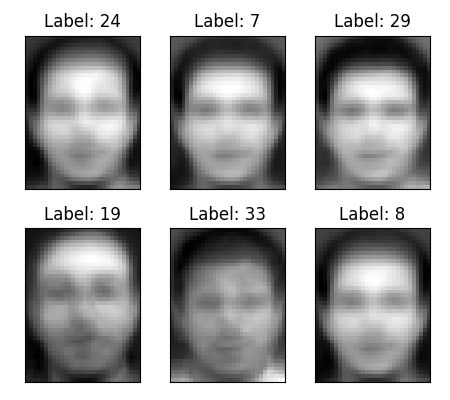
\includegraphics[width=0.7\columnwidth]{../source/orl/pictures/image-reconstructed-pca.png}
    \caption{ORL images reconstructed after PCA}
    \label{fig:orl-images-reconstructed}
\end{figure}

\begin{figure}[htbp]
    \centering
    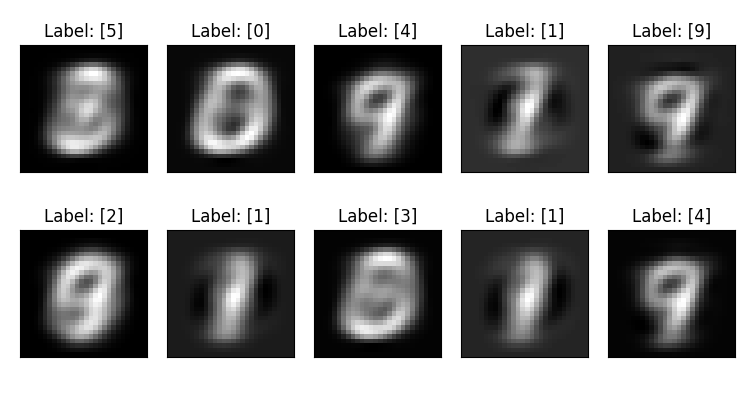
\includegraphics[width=0.7\columnwidth]{../source/mnist/pictures/image-reconstructed-pca.png}
    \caption{MNIST images reconstructed after PCA}
    \label{fig:mnist-images-reconstructed}
\end{figure}

Having the dimensions reduced to two, makes it easy to visualize the data. On Figure \ref{fig:mnist-scatter} can a scatter plot for the MNIST test data be seen. 

\begin{figure}[htbp]
    \centering
    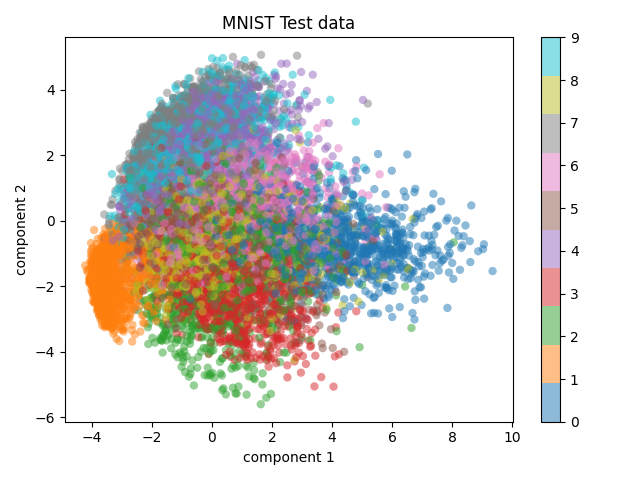
\includegraphics[width=1\columnwidth]{../source/mnist/pictures/mnist-scatter.png}
    \caption{MNIST test PCA images scatter plot}
    \label{fig:mnist-scatter}
\end{figure}

As for the ORL data set there is 40 classes, which is hard to illustrate in a single scatter plot. Therefore Figure \ref{fig:orl-scatter-first} contains the first 20 classes while Figure \ref{fig:orl-scatter-second} contains the other 20 classes. 


\begin{figure}[htbp]
    \centering
    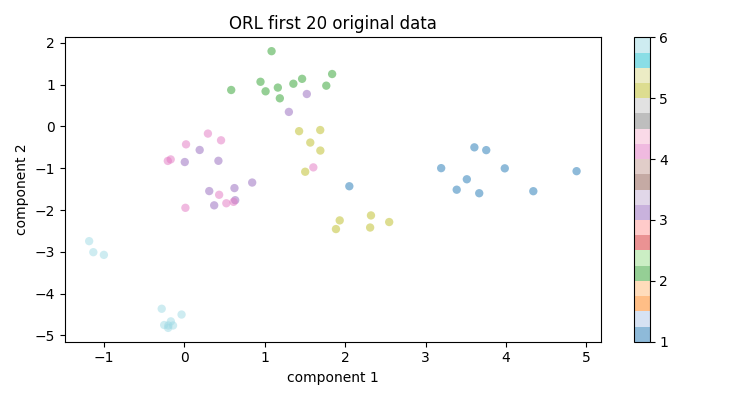
\includegraphics[width=1\columnwidth]{../source/orl/pictures/orl-scatter-original-first.png}
    \caption{ORL original PCA images first 20 classes}
    \label{fig:orl-scatter-first}
\end{figure}

\begin{figure}[htbp]
        \centering
        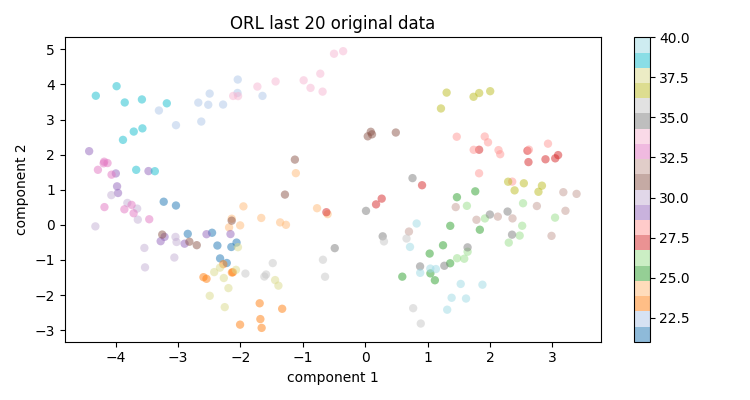
\includegraphics[width=1\columnwidth]{../source/orl/pictures/orl-scatter-original-second.png}
        \caption{ORL original PCA images last 20 classes}
        \label{fig:orl-scatter-second}
\end{figure}

\subsection{Classification}
Each classifier, for both the original data and the PCA version of the data, have their hyperparameters tuned if relevant. Afterwards the classification is performed.  
The accuracy of class predictions of the test data can be seen on Table \ref{tab:classifiers-performance}. Measurements of the time spent both training and testing can be seen for certain classifiers. 


\begin{table*}[!htbp]
    \centering
    \begin{tabular}{|l|l|l|l|l|l|} 
    \hline
    Dataset & Classifier                      & Accuracy (Raw)       & Accuracy (2d)        & Time (Raw)           & Time (2d)  \\ 
    \hline
    MNIST   & \multicolumn{1}{l}{}            & \multicolumn{1}{l}{} & \multicolumn{1}{l}{} & \multicolumn{1}{l}{} &            \\ 
    \hline
            & Nearest Class Centroid          & 82.03\%              & 43.65\%              & 0.702 s              & 0.016 s    \\ 
    \cline{2-6}
            & Nearest 2 Sub-Class Centroid    & 86.07\%              & 43.07\%              & 5.049 s              & 1.197 s    \\ 
    \cline{2-6}
            & Nearest 3 Sub-Class Centroid    & 88.24\%              & 42.39\%              & 7.918 s              & 1.918 s    \\ 
    \cline{2-6}
            & Nearest 5 Sub-Class Centroid    & 90.27\%              & 41.81\%              & 12.513 s             & 3.308 s    \\ 
    \cline{2-6}
            & Nearest Neighbor                & 96.88\%              & 42.43\%              & 14.173 s             & 0.207 s    \\ 
    \cline{2-6}
            & Perceptron with Backpropagation & 92.20\%              & 39.36\%              & 5.812 s              & 0.090 s    \\ 
    \cline{2-6}
            & Perceptron with MSE             & 86.08\%              & 32.79\%              & 5.923 s              & 0.128 s    \\ 
    \hline
    ORL     & \multicolumn{1}{l}{}            & \multicolumn{1}{l}{} & \multicolumn{1}{l}{} & \multicolumn{1}{l}{} &            \\ 
    \hline
            & Nearest Class Centroid          & 87.50\%              & 33.33\%              & 0.005 s              & 0.001 s    \\ 
    \cline{2-6}
            & Nearest 2 Sub-Class Centroid    & 94.17\%              & 40.00\%              & 0.602 s              & 0.548 s    \\ 
    \cline{2-6}
            & Nearest 3 Sub-Class Centroid    & 96.67\%              & 35.83\%              & 0.666 s              & 0.613 s    \\ 
    \cline{2-6}
            & Nearest 5 Sub-Class Centroid    & 96.67\%              & 34.17\%              & 0.828 s              & 0.748 s    \\ 
    \cline{2-6}
            & Nearest Neighbor                & 95.83\%              & 30.83\%              & 0.013 s              & 0.006 s    \\ 
    \cline{2-6}
            & Perceptron with Backpropagation & 95.83\%              & 13.33\%              & 0.073 s              & 0.015 s    \\ 
    \cline{2-6}
            & Perceptron with MSE             & 95.83\%              & 13.33\%              & 0.165 s              & 0.015 s    \\
    \hline
    \end{tabular}
    \caption{Performance of each classifier for both datasets}
    \label{tab:classifiers-performance}
\end{table*}

\subsection{Visualization}

\begin{figure*}[htbp]
        \begin{subfigure}[b]{.33\linewidth}
            \centering
            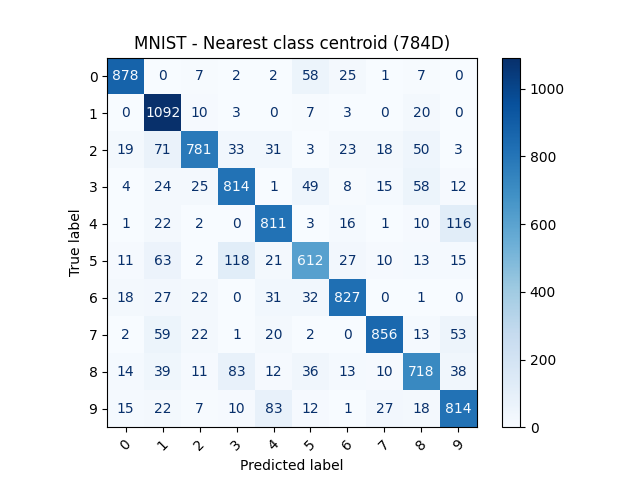
\includegraphics[width=1\linewidth]{../source/mnist/pictures/nearestClassCentroid-confusion-784d.png}
            \caption{Nearest class centroid (784D)}
            \label{fig:mnist-confusion-ncc-784}
        \end{subfigure}%
        \begin{subfigure}[b]{0.33\linewidth}
            \centering
            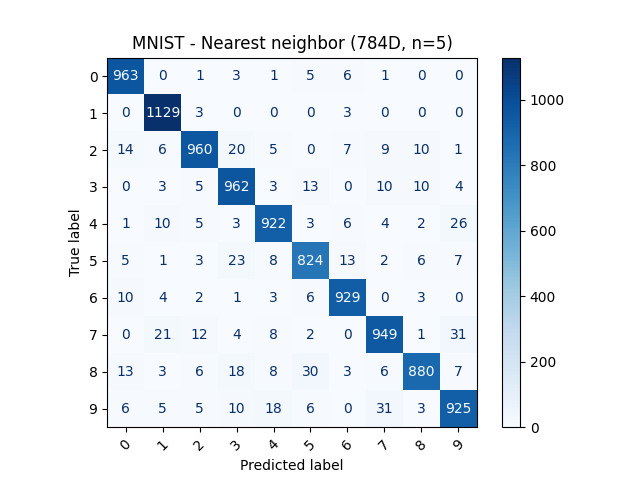
\includegraphics[width=1\linewidth]{../source/mnist/pictures/nearestNeighbor-5-confusion-784d.png}
            \caption{Nearest 5 neighbors (784D)}
            \label{fig:mnist-confusion-nn-784}
        \end{subfigure}
        \begin{subfigure}[b]{0.33\linewidth}
                \centering
                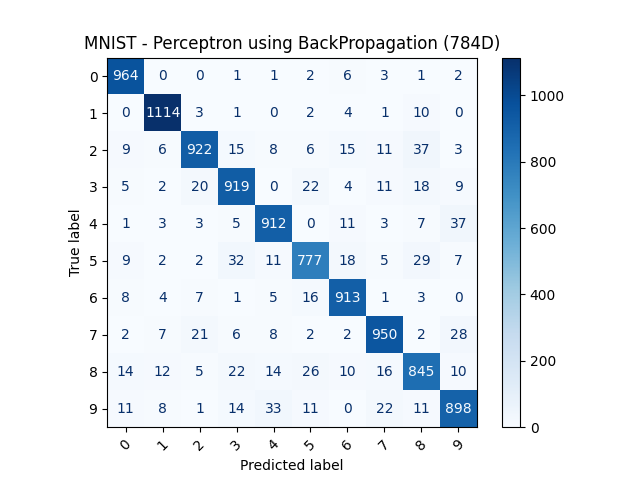
\includegraphics[width=1\linewidth]{../source/mnist/pictures/perceptronBP-confusion-784d.png}
                \caption{Perceptron using BP (784D)}
                \label{fig:mnist-confusion-pbp-784}
        \end{subfigure}

        \begin{subfigure}[b]{.33\linewidth}
                \centering
                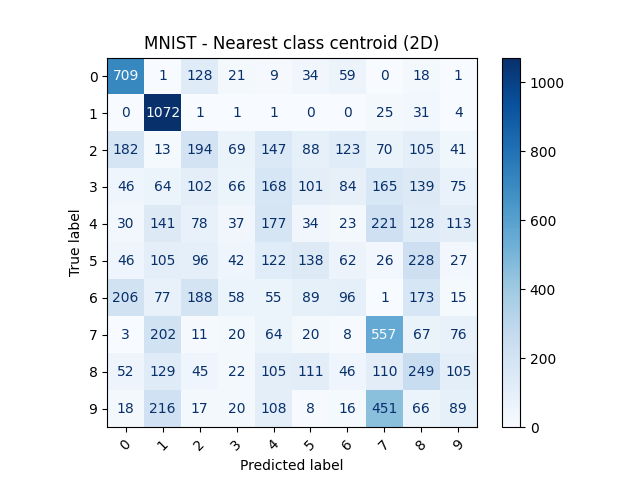
\includegraphics[width=1\linewidth]{../source/mnist/pictures/nearestClassCentroid-confusion-2d.png}
                \caption{Nearest class centroid (2D)}
                \label{fig:mnist-confusion-ncc-2}
            \end{subfigure}%
            \begin{subfigure}[b]{0.33\linewidth}
                \centering
                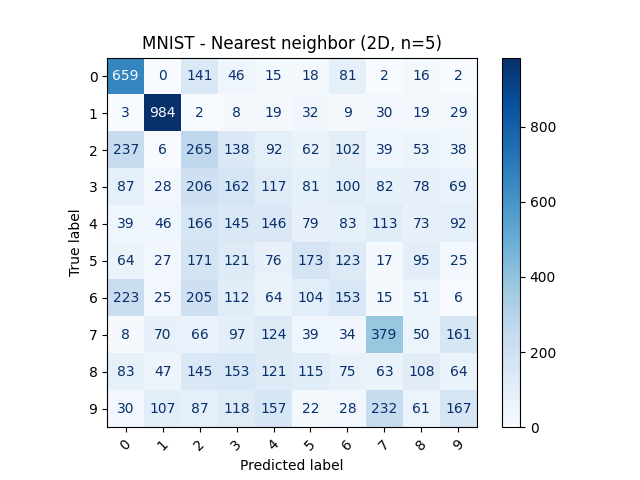
\includegraphics[width=1\linewidth]{../source/mnist/pictures/nearestNeighbor-5-confusion-2d.png}
                \caption{Nearest 5 neighbors (2D)}
                \label{fig:mnist-confusion-nn-2}
            \end{subfigure}
                \begin{subfigure}[b]{0.33\linewidth}
                    \centering
                    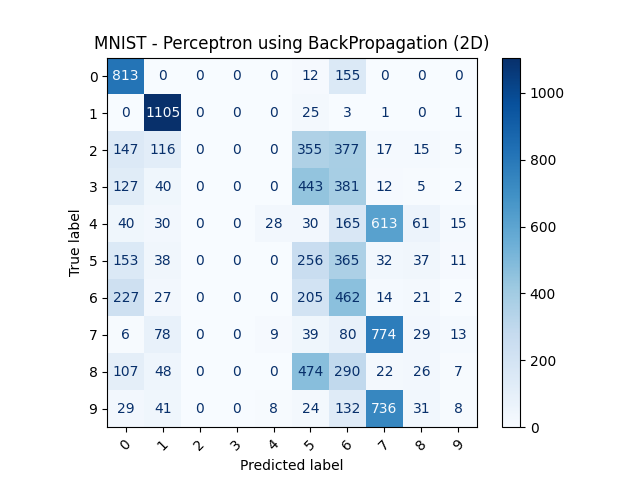
\includegraphics[width=1\linewidth]{../source/mnist/pictures/perceptronBP-confusion-2d.png}
                    \caption{Perceptron using BP (2D)}
                    \label{fig:mnist-confusion-pbp-2}
                \end{subfigure}
        \caption{Confusion Matrices - MNIST}
        \label{fig:mnist-confusion}
\end{figure*}

\begin{figure*}[htbp]
        \begin{subfigure}[b]{.33\linewidth}
            \centering
            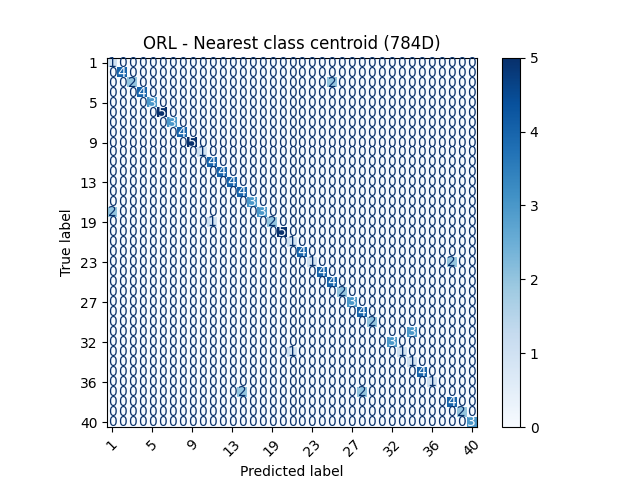
\includegraphics[width=1\linewidth]{../source/orl/pictures/nearestClassCentroid-confusion-784d.png}
            \caption{Nearest class centroid (784D)}
            \label{fig:orl-confusion-ncc-784}
        \end{subfigure}%
        \begin{subfigure}[b]{0.33\linewidth}
            \centering
            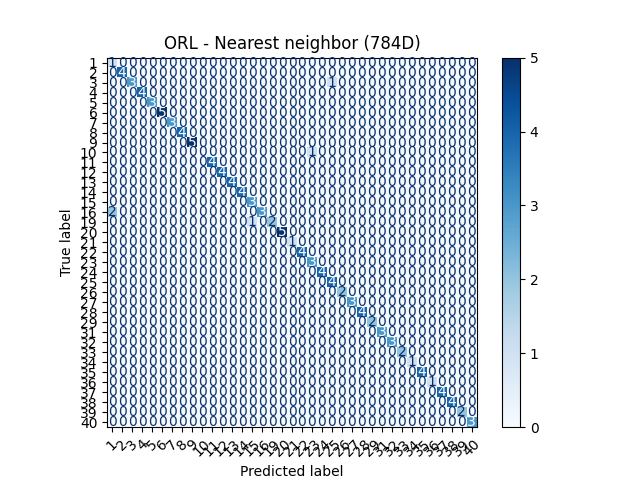
\includegraphics[width=1\linewidth]{../source/orl/pictures/nearestNeighbor-5-confusion-784d.png}
            \caption{Nearest 5 neighbors (784D)}
            \label{fig:orl-confusion-nn-784}
        \end{subfigure}
        \begin{subfigure}[b]{0.33\linewidth}
                \centering
                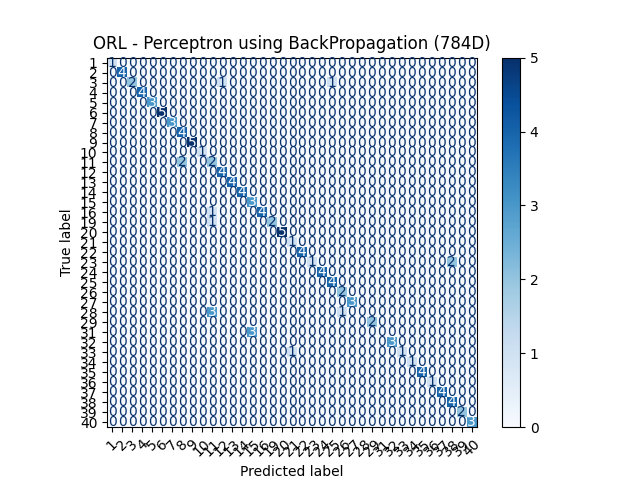
\includegraphics[width=1\linewidth]{../source/orl/pictures/perceptronBP-confusion-784d.png}
                \caption{Perceptron using BP (784D)}
                \label{fig:orl-confusion-pbp-784}
        \end{subfigure}

        \begin{subfigure}[b]{.33\linewidth}
                \centering
                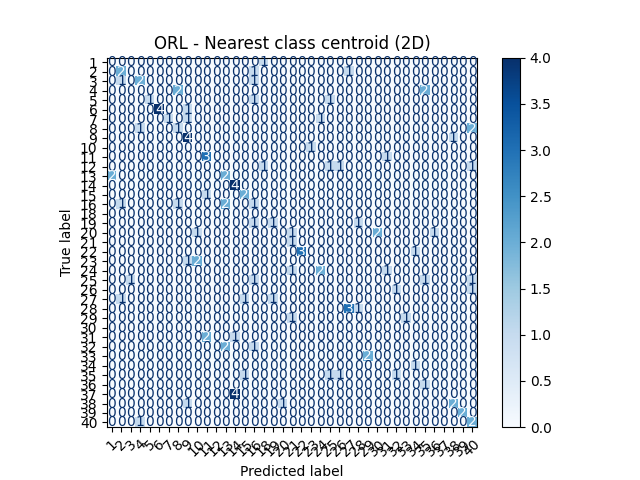
\includegraphics[width=1\linewidth]{../source/orl/pictures/nearestClassCentroid-confusion-2d.png}
                \caption{Nearest class centroid (2D)}
                \label{fig:orl-confusion-ncc-2}
        \end{subfigure}%
        \begin{subfigure}[b]{0.33\linewidth}
                \centering
                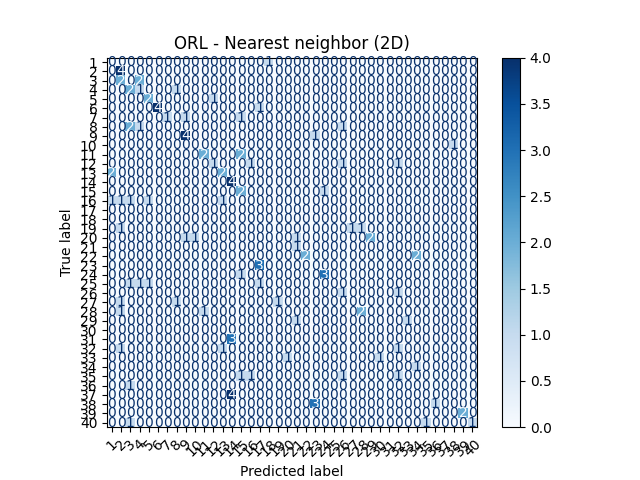
\includegraphics[width=1\linewidth]{../source/orl/pictures/nearestNeighbor-5-confusion-2d.png}
                \caption{Nearest 5 neighbors (2D)}
                \label{fig:orl-confusion-nn-2}
        \end{subfigure}
        \begin{subfigure}[b]{0.33\linewidth}
                \centering
                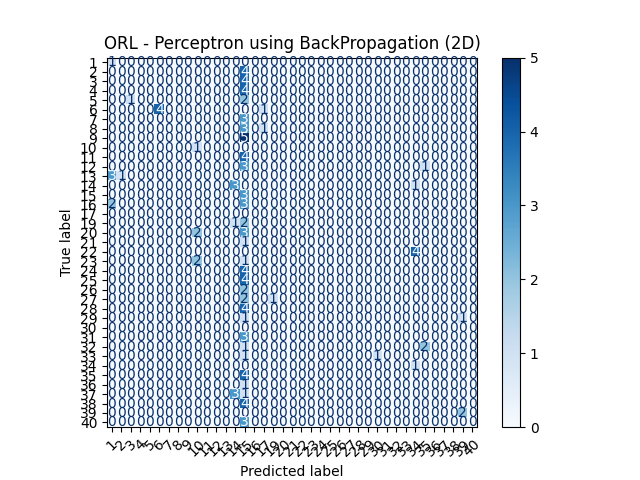
\includegraphics[width=1\linewidth]{../source/orl/pictures/perceptronBP-confusion-2d.png}
                \caption{Perceptron using BP (2D)}
                \label{fig:orl-confusion-pbp-2}
        \end{subfigure}
        \caption{Confusion Matrices - ORL}
        \label{fig:orl-confusion}
\end{figure*}

